\documentclass[11pt]{article}

\usepackage[letterpaper,margin=0.75in]{geometry}
\usepackage{booktabs}
\usepackage{graphicx}
\usepackage{listings}
\usepackage{hyperref}

\setlength{\parindent}{1.4em}

\begin{document}

\lstset{
  language=Python,
  basicstyle=\small,          % print whole listing small
  keywordstyle=\bfseries,
  identifierstyle=,           % nothing happens
  commentstyle=,              % white comments
  stringstyle=\ttfamily,      % typewriter type for strings
  showstringspaces=false,     % no special string spaces
  numbers=left,
  numberstyle=\tiny,
  numbersep=5pt,
  frame=tb,
}

\newenvironment{absolutelynopagebreak}
  {\par\nobreak\vfil\penalty0\vfilneg
   \vtop\bgroup}
  {\par\xdef\tpd{\the\prevdepth}\egroup
   \prevdepth=\tpd}

\title{Network Simulation}

\author{Cody Heffner}

\date{17 Feb. 2015}

\maketitle

\section{Preface}

This report details the experiment I ran and the results obtained as specified by the Reliable Transport Lab in the BYU CS 460 class taught by Dr. Zappala. The project specifications can be found \href{http://cs460.byu.edu/winter-2015/labs/reliable-transport}{here}.

The experiment requires heavy use of a network simulator to test different network scenarios. The network simulator I used is Dr. Zappala's \href{https://github.com/zappala/bene}{Bene}, written in Python. All my simulation examples shown will be tailored towards use for that simulator.

\section{Summary}

The goal of the experiment was to show that reliable transport of data is possible and that dynamic retransmission timers work and are effective. The first section of the report describes how I implemented reliable transport. The second section discusses my implementation of a dynamic retransmission timer and includes data and analysis of my implementation.

\section{Reliable Transport}

Reliable transport in TCP is simply achieved by the sender marking each segment with the number of the starting byte of data. In other words, if the sender is sending bytes 30-50, the sender marks the segment with the value \emph{30}. When the receiver receives a segment, it replies with the value of the next byte it expects to receive. When the sender receives bytes 30-50 (after already obtaining bytes 1-29), it replies with a value of \emph{51} because that is the next byte it doesn't have yet. 

This is a reliable method of transport because the receiver is constantly letting the sender know what to send next. If the first in a bunch of packets sent gets lost, the receiver simply buffers the future packets and lets the receiver know exactly which portion of data is missing.

By coding this behavior into my TCP implementation, I was able to acheive reliable transport and send files in a variety of unreliable networks. The following blocks show my experimental data in 10 Mbps networks with propagation delays of 10 ms, varying window sizes, varying files, and varying loss rates. The files used were all obtained from Zappala's Bene repository.

\vspace{0.5cm}
\begin{absolutelynopagebreak}
\begin{tabular}{rclr}
  \toprule
  Window Size & Loss Rates & File Name & Transfer Time (s) \\
  \midrule
  3000 &  0\% & test.txt &  0.088 \\
  3000 & 10\% & test.txt &  2.106 \\
  3000 & 20\% & test.txt &  4.106 \\
  3000 & 50\% & test.txt & 34.166 \\

  10,000 &  0\% & internet-architecture.pdf &   1.451 \\
  10,000 & 10\% & internet-architecture.pdf &  49.361 \\
  10,000 & 20\% & internet-architecture.pdf &  88.019 \\
  10,000 & 50\% & internet-architecture.pdf & 420.112 \\
  \bottomrule
\end{tabular}
\end{absolutelynopagebreak}
\vspace{0.5cm}

All outputs received the message \emph{File transfer correct!} as the last line, indicating that all bytes were received.

\section{Dynamic Retransmission Timer}

The dynamic retransmission timer was implemented by recalculating the timeout value whenever an ack was received and resetting the timeout value whenever a retransmission occured. The timeout value was obtained by keeping track of the interval between when a packet was sent and that packet's ack was received. That value was multiplied by an alpha value and added to the product of 1-alpha and the old retransmission timer. The timer was then set to be that value if it was between the minimum and maximum times, which are 200 ms and 1 second, respectively.

The following table shows the updated file transfer times. This table should be compared directly to the corresponding table in the previous section.

\vspace{0.5cm}
\begin{absolutelynopagebreak}
\begin{tabular}{rclr}
  \toprule
  Window Size & Loss Rates & File Name & Transfer Time (s) \\
  \midrule
  3000 & 00\% & test.txt &  0.088 \\
  3000 & 10\% & test.txt &  0.757 \\
  3000 & 20\% & test.txt &  2.479 \\
  3000 & 50\% & test.txt & 10.683 \\

  10,000 & 00\% & internet-architecture.pdf &   1.451 \\
  10,000 & 10\% & internet-architecture.pdf &  26.480 \\
  10,000 & 20\% & internet-architecture.pdf &  46.874 \\
  10,000 & 50\% & internet-architecture.pdf & 395.769 \\
  \bottomrule
\end{tabular}
\end{absolutelynopagebreak}
\vspace{0.5cm}

By inspection, the files transferred significantly faster, especially when loss was kept low. It is worth pointing out that the file transfer did not speed up significantly with the pdf file on a 50\% loss network. I theorize this is because so many packets were lost that the retransmission timer was kept near the maximum value. File transfer speed saw the most increase (a 100\% gain on 10 and 20 percent loss networks) from a dynamic transmission timer when loss was kept low, no more than around 20\%. 

The following table shows output from a script I wrote to parse the output to find the average wait time between a packet being sent and a retransmission timer firing.

\vspace{0.5cm}
\begin{absolutelynopagebreak}
\begin{tabular}{rclr}
  \toprule
  Window Size & Loss Rates & File Name & Avg Retransmission Time (s)\\
  \midrule
  3000 & 00\% & test.txt & 0 \\
  3000 & 10\% & test.txt & 0.658 \\
  3000 & 20\% & test.txt & 0.780 \\
  3000 & 50\% & test.txt & 0.953 \\

  10,000 & 00\% & internet-architecture.pdf & 0 \\
  10,000 & 10\% & internet-architecture.pdf & 0.443 \\
  10,000 & 20\% & internet-architecture.pdf & 0.577 \\
  10,000 & 50\% & internet-architecture.pdf & 0.925 \\
  \bottomrule
\end{tabular}
\end{absolutelynopagebreak}
\vspace{0.5cm}

As can be seen, the retransmission timer approaches 0.2 seconds as loss approaches 0\%, and the timer approaches 1 second as loss increases, as theorized.

\section{Experiments}

The experiments conducted set the bandwidth of a two-node network to 10 Mbps with a propagation delay of 10 ms, a queue size of 100, and a loss rate of 0\%. I then transferred the \emph{internet-architecture.pdf} file using window dizes of 1000, 2000, 5000, 10000, 15000, and 20000 bytes. I computed teh throughput of the transfer as the total bits sent divided by the total time to send the file, measured from the start of the simulation to when the last segment was received. I computed the average queueing delay of all segments sent, then plotted the throughput and the average queueing delay as a function of the window size on two separate graphs.

The following graph shows the average queue duration as a function of window size as determined by the experiment. The queue times were determined by subtracting the propagation and transmission delay from the total time to send, then dividing that value by the number of packets into which the file was split.

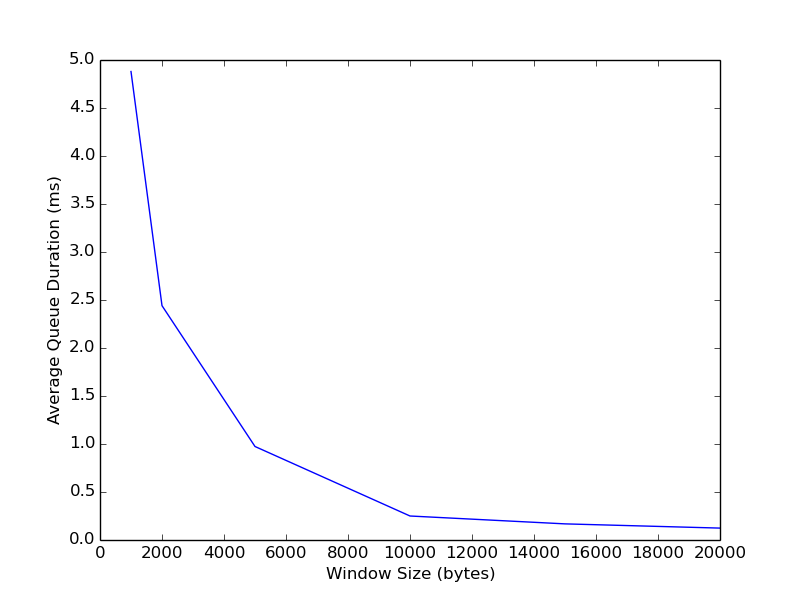
\includegraphics[width=17cm]{outputs/lab2_queue.png}

The queue time increases exponentially as the window size decreases. This is the expected output because if window size is small, the sender will be holding the data for a longer period of time in its buffer.

The following graph shows the calculated throughput of the network as window size increases. The throughput was determined as the number of bits sent (the file size) divided by the time to send in seconds.

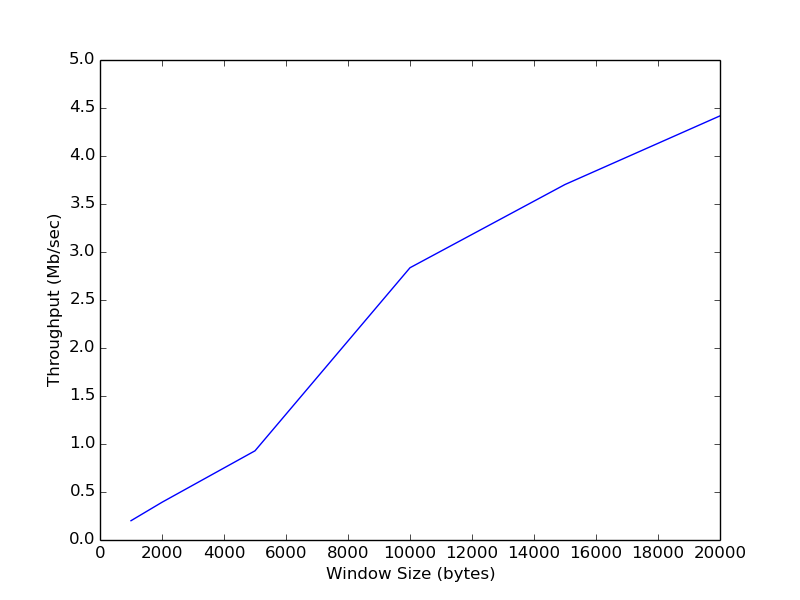
\includegraphics[width=17cm]{outputs/lab2_throughput.png}

Throughput is approximately linearly increased as window size increases. However, the maximum bandwidth of the line is 10 Mbps, so there is a hard cap to throughput.

\end{document}
